% Compile with XeLaTeX. The figure is schematic, not empirical data.
\documentclass[tikz,border=2pt]{standalone}
\usepackage{fontspec}
\IfFontExistsTF{Times New Roman}{\setmainfont{Times New Roman}}{%
  \IfFontExistsTF{Tinos}{\setmainfont{Tinos}}{\setmainfont{Liberation Serif}}}
\usepackage{unicode-math}
\IfFontExistsTF{STIX Two Math}{\setmathfont{STIX Two Math}}{%
  \IfFontExistsTF{STIX Math}{\setmathfont{STIX Math}}{\setmathfont{Latin Modern Math}}}
\usetikzlibrary{arrows.meta,calc}

% Colors shared with the rank-partition figures.
\definecolor{ink}{HTML}{253139}
\definecolor{linegray}{HTML}{65747E}
\definecolor{guidegray}{HTML}{9CA9B1}
\definecolor{bandfill}{HTML}{D5E6F1}
\definecolor{overlapfill}{HTML}{F7E6AF}
\definecolor{boundline}{HTML}{52758A}
\definecolor{intervalink}{HTML}{9B752B}
\tikzset{font=\fontsize{9.5}{11}\selectfont,text=ink,
  labelsmall/.style={font=\fontsize{8.6}{10}\selectfont},
  axisarrow/.style={-{Stealth[length=3.5pt,width=4pt]},line width=.7pt,draw=ink},
  bound/.style={draw=boundline,line width=.9pt},
  truecdf/.style={draw=ink,line width=.85pt,dash pattern=on 3pt off 2pt},
  guide/.style={draw=guidegray,line width=.45pt,densely dashed},
  leader/.style={draw=linegray,line width=.45pt,-{Stealth[length=2.5pt,width=2.6pt]}},
  interval/.style={draw=intervalink,line width=1.3pt}}

\begin{document}
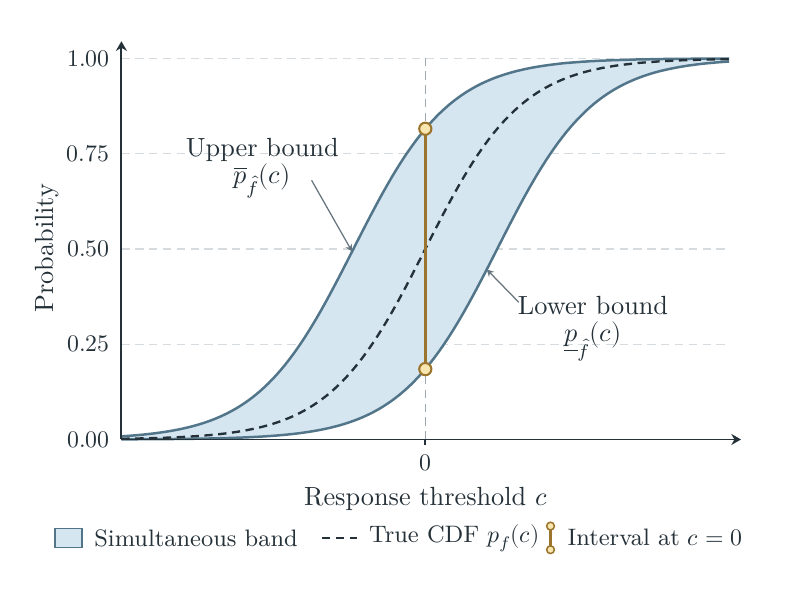
\begin{tikzpicture}[x=1cm,y=1cm]
  \path[use as bounding box] (0,0) rectangle (9.4,6.82);
  % All three curves share a slope and differ only by a horizontal shift.
  % This guarantees monotonicity and L(c) <= F(c) <= U(c) for every real c.
  \pgfmathdeclarefunction{uppercdf}{1}{\pgfmathparse{1/(1+exp(-1.35*(#1+1.1)))}}
  \pgfmathdeclarefunction{lowercdf}{1}{\pgfmathparse{1/(1+exp(-1.35*(#1-1.1)))}}
  \pgfmathdeclarefunction{truecdf}{1}{\pgfmathparse{1/(1+exp(-1.35*#1))}}
  \pgfmathsetmacro{\plo}{lowercdf(0)}
  \pgfmathsetmacro{\phi}{uppercdf(0)}

  % Data coordinates: the horizontal axis is c, not an empirical data scale.
  \begin{scope}[shift={(5.05,1.59)},x=.83cm,y=4.84cm]
    % Light horizontal reference guides.
    \foreach \p/\lab in {0/0.00,.25/0.25,.5/0.50,.75/0.75,1/1.00}{
      \draw[draw=guidegray!42,line width=.42pt,densely dashed] (-4.65,\p)--(4.65,\p);
      \node[anchor=east,labelsmall,inner sep=2pt] at (-4.74,\p) {$\lab$};
    }
    % The confidence band is filled before the boundary curves are drawn.
    \fill[bandfill]
      plot[domain=-4.65:4.65,samples=150] (\x,{uppercdf(\x)})
      -- plot[domain=4.65:-4.65,samples=150] (\x,{lowercdf(\x)}) -- cycle;
    % The c=0 reference guide sits underneath the curves and interval.
    \draw[guide] (0,0)--(0,1);
    \draw[bound] plot[domain=-4.65:4.65,samples=150] (\x,{uppercdf(\x)});
    \draw[bound] plot[domain=-4.65:4.65,samples=150] (\x,{lowercdf(\x)});
    \draw[truecdf] plot[domain=-4.65:4.65,samples=150] (\x,{truecdf(\x)});
    % The highlighted original scalar interval is exactly the slice at c=0.
    \draw[interval] (0,\plo)--(0,\phi);
    \node[circle,draw=intervalink,fill=overlapfill,inner sep=0pt,minimum size=4.4pt,line width=.75pt] at (0,\plo) {};
    \node[circle,draw=intervalink,fill=overlapfill,inner sep=0pt,minimum size=4.4pt,line width=.75pt] at (0,\phi) {};
    \draw[axisarrow] (-4.65,0)--(4.83,0);
    \draw[axisarrow] (-4.65,0)--(-4.65,1.045);
    \draw[ink,line width=.6pt] (0,0)--(0,-.014);
    \node[anchor=north,labelsmall,inner sep=2pt] at (0,-.023) {$0$};
    % Short leaders terminate exactly on the mathematical curves.
    \draw[leader] (-1.74,.68)--(-1.12,{uppercdf(-1.12)});
    \draw[leader] (1.43,.36)--(.94,{lowercdf(.94)});
  \end{scope}

  % Direct labels, kept outside the shaded corridor and away from the curves.
  \node[align=center,inner sep=0pt] at (2.98,5.04)
    {Upper bound\\[-1pt]$\overline p_{\hat f}(c)$};
  \node[align=center,inner sep=0pt] at (7.18,3.00)
    {Lower bound\\[-1pt]$\underline p_{\hat f}(c)$};
  \node[rotate=90] at (.24,4.02) {Probability};
  \node at (5.05,.84) {Response threshold $c$};

  % The compact key mirrors the legend style of the joint partition figure.
  \fill[bandfill] (.35,.22) rectangle (.69,.46);
  \draw[boundline,line width=.55pt] (.35,.22) rectangle (.69,.46);
  \node[anchor=west,labelsmall,inner sep=2pt] at (.77,.34) {Simultaneous band};
  \draw[truecdf] (3.74,.34)--(4.18,.34);
  \node[anchor=west,labelsmall,inner sep=2pt] at (4.26,.34) {True CDF $p_f(c)$};
  \draw[interval] (6.64,.19)--(6.64,.49);
  \foreach \y in {.19,.49} {\node[circle,draw=intervalink,fill=overlapfill,inner sep=0pt,minimum size=2.8pt,line width=.55pt] at (6.64,\y) {};}
  \node[anchor=west,labelsmall,inner sep=2pt] at (6.78,.34) {Interval at $c=0$};
\end{tikzpicture}
\end{document}
